\documentclass{article}

\topmargin  0.0in
\headheight  0.15in
\headsep  0.15in
\footskip  0.2in
\textheight 8.45in

\oddsidemargin 0.56in
\evensidemargin \oddsidemargin
\textwidth 5.8in

\usepackage{clrscode}
\usepackage{graphicx}
%%\input{epsf}

\pagestyle{myheadings}
\markright{\bf The Dependency Graph Generation Algorithm}

\begin{document}

\title{The Dependency Graph Generation Algorithm}

\author{ Yang Zhang \\
\it fz15@erc.msstate.edu}

\maketitle

% example of figure including code
%\begin{figure}[htbp]
%  \centerline{ \epsfxsize=5.5in \epsfbox{figures/constructs.eps}}
% \caption{Four Basic Container Categories}
% \label{constructs}
%\end{figure}

\section{Introduction}

This document provides an overview of the dependency graph generation
algorithm for the Loci framework. It also discusses some of the
backgrounds, strategies, and considerations in developing the
algorithm.

\section{The Main Idea}
\label{sec:main}
The purpose of the dependency graph is to set up the control and data
flows from the given known facts to the user queried facts. It is
required that the rule database, the given facts, and the target
(queried) facts are known before we start to generate the dependency
graph. The dependency graph is a directed (possibly cyclic) graph
which partially orders all the necessary facts and rules needed to
assemble an application program. 

In the current version of Loci, a recursive backward searching
algorithm is used to generate the dependency graph. Being recursive
means that the algorithm works by dividing the task into small similar
problems. Being backward searching means the algorithm works by
always looking back from the targets that we are about to compute. 

The main complications of the algorithm come from the presence of
iteration. In Loci, iterations are defined by a set of rules. Namely
the build rules which initialize the iteration, the advance rules
which inductively compute the contents of the iteration, and the
collapse rules which terminate the iteration. Each iteration has a
unique time identity associated with it. This time identity represents
the time level that the particular iteration is operating. Multiple
iterations are organized into a hierarchy, with the stationary time
(things that do not iterate) being the root and the deepest iterations
being the leafs. In this document, we refer to an iteration's 
{\it parent} as the iteration with just one level higher in the
hierarchy as the former iteration. In other words, the parent
iteration is one level shallower than its children, and its time level
is also one level
before its children's. For example, $\{n\}, \{n,it\}, \{n,it,igs\}$
form a hierarchy, with $\{n\}$ being the most shallow iteration and
$\{n,it,igs\}$ the deepest.

If two iterations stay at the same level in the hierarchy, they are
said to be independent of each other. Independent iterations rarely
cause complications in generating the dependency graph. It is the
nested iterations that are the source of intricacy. 

If an application has no iterations, then its control structure is a
plain directed acyclic graph (Dag). When we build its dependency
graph, we start from the queried targets and looking back for all the
rules that generate the targets. In order to be able to execute
these rules, their sources must be known. Then in turn, we start again
from those sources and continue to look back until we hit those given
facts. This is the main idea of backward searching. 

In the backward searching, a rule's sources are called the rule's
{\it requests}. These requests are of crucial to the searching and the
correctness of the final dependency graph. If at any time, we pass an
incorrect requests set back in searching, then the graph being built
will likely to be seriously flawed. 

Since in Loci, iterations are defined by a set of rules, we will first
need to recognize all the iterations in the rule database before we
build the dependency graph. Because iterations require extra controls,
we therefore cannot treat the set of rules that make up the iteration
as other concrete rules. And since iterations accept inputs and
compute one or more targets, they act as other rules. We instead
regard them as super rules or black-box rules in dependency graph
building. Therefore, once we recognized all iterations, in the
backward searching, if we hit an iteration, we will also need to
collect its requests and pass them back.

The complications of iteration enter here. Because of the way that
iterations are defined in Loci, we do not precisely know what an
iteration's requests is after we recognize it. It is true that the
build rules' sources of an iteration are the requests, but it may only
contribute partly to the whole requests. Because iterations will
iterate, the advance part therefore plays an important role in the
iteration. It is possible (and almost certainly) that some facts
will be brought in directly into the advance part. Those facts are
also required to be in the requests set of that iteration. The problem
is at the time when we recognizing the iteration from the rule
database, we do not yet know exactly what are the source facts for the
advance part. Because at that time, we only know the advance
rules and the advance rules may require other rules in computing
them. This is due to Loci's declarative nature. We actually need to
search back to know precisely what we need. And in the advance part,
the facts and rule promotion and the I/O handle present the most
complications (see section \ref{sec:consider} for detailed
discussion).

The recursive nature of the dependency graph generation algorithm
comes in with the treatment of iterations. Because we need to know
precisely the requests of an iteration, we will need to process it
first. Therefore, when we see an iteration during the
backward searching, we trap into it and apply the backward searching
again on the iteration to find its requests. Applying backward
searching to an iteration also means to build the dependency graph for
that iteration. Hence this process is also referred to as
{\it iteration instantiation}. This process is also recursive because
an iteration might contain arbitrary child iterations. Instantiating
an iteration is more than backward searching, it also involves an
initialization phase that gathers necessary information. 

Simply put, the dependency graph generation algorithm alternates
between backward requests passing and iteration instantiation in the
rule database's time level hierarchy.

\section{The Algorithm}
\label{sec:algorithm}
The main source code of implementation is \texttt{depend\_graph2.cc} 
in \texttt{src/System} directory. The algorithm presented here is
adapted from the source code. Some underlying data-structures may
changed in the algorithm descriptions here, but the essential steps
are the same. Whenever possible, correspondences and differences to
the source code will be given. The actual source code will be typeset
in \texttt{typewriter} font, and the pseudo-code (the algorithm) will
be typeset in \textsc{small caps} font. 

We will first point out the handling\footnote{We mean to generate the
  rule at appropriate place in the dependency graph.} of the three
  types of internal
recurrence rules in Loci. Namely the \texttt{priority} rule, the
\texttt{generalize} rule, and the \texttt{promote} rule. Each of them
are handled in a different level in the graph generation
algorithm. The priority rule is handled at the lowest level
  in the algorithm (in the \proc{Add-To-Graph} function below in the
  algorithm). Whenever we want to add a concrete rule to the
  graph, we make a check to see if any of the rule's target facts are
  involved in any priority information. If true, we append the
  necessary priority rule here. The source code that responds this is
  the \texttt{invoke\_rule\_wp} function. The generalize rule is
  handled in the initialization phase of an iteration (the
  \texttt{iteration::init} method). The promote
  rule is handled during the backward searching phase (the
  \texttt{create\_graph} function). They will be
  described in detail below.

As mentioned in section~\ref{sec:main}, before the graph gets built, a
classification of the rule database is first performed. In the
classification, all iteration related rules are singled out. The rules
that define an iteration are then replaced by a fictitious internal
rule named \texttt{iterating\_rule}. The source facts of this rule is
the source facts of all the build rules and the target facts being the
collapse rules' targets. Then we put all the remaining rules
(stationary time rules and time specific rules) and these possible
\texttt{iterating\_rule} into a directed graph. This graph is referred
to as \texttt{rule\_graph} in the source code and represents the
entire rule database and also is the basis for backward
searching. Here, we should point out an important fact:
an~\texttt{iterating\_rule} itself may be an advance rule for its
parent iteration. Therefore, it is possible that not all of the
\texttt{iterating\_rule}s will be in the the \texttt{rule\_graph}
since all the rules that define an iteration are taken off from the
\texttt{rule\_graph}. The code that corresponds to the
classification is \texttt{classify\_ruledb} and
\texttt{create\_iteration\_rep} functions. The algorithm for
classification is rather straightforward and should be
obvious from reading relative source code. The key steps are Loci
data-structure operations.

\sloppy{
The central part of the implementation is the \texttt{iteration::init}
method, the \texttt{instantiate\_iteration} function, and the
\texttt{create\_graph} function in the source code. The algorithm is
described in \proc{Iter-Init}, \proc{Instantiate-Iter}, and
\proc{Create-Graph} respectively. 

}%end of sloppy

First, we will need to point out their relations. The whole dependency
graph generation algorithm is referred to as recursive backward
searching algorithm. Hence, they are recursive algorithms, and more
specifically, they are mutually recursive. Their relations are given
as following:

\begin{codebox}
\Procname{$\proc{Init-Iter}()$}
\li  \proc{Instantiate-Iter}()
\end{codebox}

\begin{codebox}
\Procname{$\proc{Instantiate-Iter}()$}
\li  \proc{Init-Iter}()
\li  \proc{Create-Graph}()
\end{codebox}

\begin{codebox}
\Procname{$\proc{Create-Graph}()$}
\li  \proc{Instantiate-Iter}()
\end{codebox}

Among these functions, \proc{Create-Graph} is the most basic one and
is the entry point of the whole graph building algorithm. The basic
idea of this function is: given a time level and a set of search
requests, \proc{Create-Graph} looks back in the \texttt{rule\_graph},
invoking necessary rules and collecting rule requests until it cannot
proceed. In the searching, when it sees an iteration (an
\texttt{iterating\_rule}), it calls
\proc{Instantiate-Iter} to process the iteration
first. \proc{Create-Graph} also handles the rule promotion and
fact promotion. The promotion concept is created for
iterations, please see section~\ref{sec:consider} for detail. The
basic idea for promotion is: For each iteration, we compute a set of
facts whose contents will change during iteration, they are referred
to as {\it iteration volatile fact}. For those facts whose contents do
not change in iteration, we refer them as 
{\it iteration static fact}. For any iteration volatile fact, all
possible rule promotions are added while fact promotions are
forbidden. For any iteration static fact, only fact promotion is
allowed. 

\begin{codebox}
\Procname{$\proc{Create-Graph}(rg,sr,tlevel,dg)$}
\li $\id{requests} \gets \const{nil}$
\li $\id{rgt} \gets \proc{Transpose}(rg)$\>\>\>\>\>\>\Comment Transpose
the \texttt{rule\_graph} for backward searching
\li \Comment Get the iteration volatile facts for time level \id{tlevel}
\li $\id{vfacts} \gets \proc{Get-Volatile-Facts}(tlevel)$
\li $\id{working-facts} \gets sr$
\li \While $\id{working-facts} \ne \const{nil}$
\li   \Do
         $\id{visited-facts} \gets \id{visited-facts} + \id{working-facts}$
\li      $\id{next} \gets \const{nil}$
\li      \For $\id{f} \in \id{working-facts}$
\li        \>\Comment Get all rules that generate this fact
\li        \Do
              $\id{pre-rules} \gets \proc{Get-Next-Rules}(rgt,f)$
\li           $\id{pre-rules} \gets \id{pre-rules} - \id{visited-rules}$
\li           \For $\id{r} \in \id{pre-rules}$ 
\li             \Do
                 \If $\proc{Is-Iterating-Rule}(r)$
\li                 \Then
                   $\id{iter-requests} \gets \proc{Instantiate-Iter}(rg,r)$
\li                $\id{next} \gets \id{next} + \id{iter-requests}$
\li                 \Else
                   $\proc{Add-To-Graph}(r,dg)$
\li                $\id{next} \gets \id{next} + \proc{Get-Next-Facts}(rgt,f)$
                 \End
              \End
\li           $\id{visited-rules} \gets \id{visited-rules} + \id{pre-rules}$
\li           \If $\id{f} \in \id{vfacts}$
\li              \Then $\id{prules} \gets \proc{Get-Promote-Rules}(rgt,f)$
\li                    $\id{prules} \gets \id{prules} - \id{visited-rules}$
\li                    $\proc{Add-To-Graph}(prules,dg)$
\li               $\id{next} \gets \id{next} +~\proc{Get-Sources}(prules)$
\li              \Else $\id{fp} \gets \proc{Get-Parent-Fact}(f,tlevel)$
\li                    $\proc{Fact-Promote}(fp,f,dg)$
\li                    $\id{requests} \gets \id{requests} + \id{fp}$
              \End
         \End
\li      $\id{next} \gets \id{next} - \id{visited-facts}$
\li      $\id{working-facts} \gets \id{next}$
    \End
\li \Return $\id{requests}$
\end{codebox}

\proc{Create-Graph} takes four parameters, \id{rg} is the
\texttt{rule\_graph}, \id{sr} is the initial search 
requests\footnote{Do not be confused by the iteration's requests and
  the search requests. The iteration's requests is the precondition
  for an iteration. In the backward searching, it will be passed to
  the iteration's parent level to continue the searching. While the
  iteration's search requests could be regarded as the iteration's
  postcondition (although it may not actually be). It is used to start
  the searching for the iteration.},
\id{tlevel} is the time level, and \id{dg} is the dependency graph
about to be generated. As pointed out previously, this is the entry
point of the whole algorithm. Therefore, after the rule database is
classified, we call \proc{Create-Graph} with \id{rg} being the
\texttt{rule\_graph}, \id{sr} being the user queried facts,
\id{tlevel} equals the stationary time, and \id{dg} being the empty
dependency graph represents the whole application. In this
implementation, in all the successive \proc{Create-Graph} calls, the
\id{rg} argument is always the \texttt{rule\_graph}. Because as we
pointed out, it represents the whole rule database and is the basis
for searching. All the auxiliary
function calls in \proc{Create-Graph} should be self-clear from their
names. Upon exit, \proc{Create-Graph} returns a set of facts. This set
(the \id{requests} in the algorithm) represents the requests (only
partially) that \id{tlevel} asked for its parent level and will be
passed back to its parent level. Each call to \proc{Create-Graph} will
build a dependency graph for the specified time level. At the end, we
will need union all of these graphs to get the complete
final dependency graph. 

In \proc{Create-Graph}, when an \texttt{iterating\_rule} is seen,
\proc{Instantiate-Iter} will be triggered. Its central task is to
create the dependency graph for the iteration and complete the
iteration requests to its parent level. The \id{requests} returned in
\proc{Create-Graph} represents the facts needed in the advance
path. For an iteration, the sources of all the build rules are also
part of the requests. Since all the build rules are not in
\texttt{rule\_graph}, they will not be reached in
\proc{Create-Graph}. Hence, in~\proc{Instantiate-Iter}, we need to
union these two sets together to get the complete iteration
requests. Procedure~\proc{Instantiate-Iter} takes two arguments:
\id{rg} is the \texttt{rule\_graph} and \id{r} is the iteration being
instantiated. 

\begin{codebox}
\Procname{$\proc{Instantiate-Iter}(rg,r)$}
\li  $\id{tlevel} \gets \proc{Get-Time-Level}(r)$
\li  $\proc{Init-Iter}(rg,tlevel)$
\li  $\id{sr} \gets \proc{Get-Search-Requests}(tlevel)$
\li  $\id{dg} \gets \proc{Get-Iteration-Graph}(tlevel)$
\li  $\id{rs} \gets \proc{Get-Build-Sources}(tlevel)$
\li  $\id{rs} \gets \id{rs} +~\proc{Create-Graph}(rg,sr,tlevel,dg)$
\li  \Return $\id{rs}$
\end{codebox}

In order to create the iteration dependency graph, we will need to
know the initial search request of that iteration. This is computed in
\proc{Init-Iter}. Along with this, \proc{Init-Iter} also computes the
important iteration volatile facts, sets up the generalize rules,
creating output handling and time variable, and invoking build,
advance, and collapse rules in the iteration graph. 

\begin{codebox}
\Procname{$\proc{Init-Iter}(rg,tlevel)$}
\li  $\id{dg} \gets \const{empty}$\>\>\>\>\Comment Initialize the
iteration dependency graph
\li  $\id{vfacts} \gets \const{nil}$\>\>\>\>\Comment Initialize the
iteration volatile facts
\li  $\proc{Add-Generalize-Rules}(dg,tlevel)$
\li  $\id{tvar} \gets \proc{Create-Time-Variable}(tlevel)$
\li  $\id{output} \gets \proc{Create-Output}(tlevel)$
\li  $\id{vfacts} \gets \id{vfacts} + \id{tvar}$
\li  \For $r \in \id{build-rules}$
\li    \Do
          $\proc{Add-To-Graph}(r,dg)$
\li       $\id{vfacts} \gets \id{vfacts} +~\proc{Get-Targets}(r)$
     \End
\li  $\id{col-inputs} \gets \const{nil}$
\li  \For $r \in \id{collapse-rules}$
\li    \Do
          $\id{col-inputs} \gets \id{col-inputs}
           +~\proc{Get-Sources}(r)$
\li       $\proc{Add-To-Graph}(r,dg)$
     \End
\li  $\id{adv-inputs} \gets \const{nil}$
\li  \For $r \in \id{advance-rules}$
\li    \Do
          $\id{vfacts} \gets \id{vfacts} + \proc{Get-Targets}(r)$
\li       \If $\proc{Is-Iterating-Rule}(r)$
\li         \Then
               $\id{adv-inputs} \gets \id{adv-inputs} + 
               \proc{Instantiate-Iter}(rg,r)$
\li         \Else
               $\id{adv-inputs} \gets \id{adv-inputs} +
               \proc{Get-Sources}(r)$
\li            $\proc{Add-To-Graph}(r,dg)$
          \End
     \End
\li  $\id{irule} \gets \proc{Create-Looping-Rule}$\label{li:irule}
\li  $\proc{Add-To-Graph}(irule,dg)$
\li  $\id{sr} \gets \id{col-inputs}$\>\>\>\>\Comment The searching requests
\li  $\id{sr} \gets \id{sr} + \id{adv-inputs}$
\li  $\id{vfacts} \gets \proc{Compute-Volatile-Facts}(rg,vfacts,tlevel)$
\li  \If $\id{output} \in \id{vfacts}$\label{li:output1}
\li    \Then
          $\id{sr} \gets \id{sr} + \id{output}$\label{li:output2}
     \End
\li  \Comment Save the iteration dependency graph, searching requests, and the
\li  \Comment iteration volatile facts into data-structure
associated with \id{tlevel}
\li  $\proc{Save-Time-Info}(dg,sr,vfacts,tlevel)$
\end{codebox}

Procedure~\proc{Init-Iter} takes two arguments, \id{rg} is the
\texttt{rule\_graph} and \id{tlevel} is the iteration's time level.
There are several keys in \proc{Init-Iter}. First, \id{sr} in the
algorithm means the searching requests of that iteration. Because we
use backward searching, we will need to supply an initial set of facts
to start up. For the stationary time graph, as discussed previously,
the searching requests is just the user queried facts. For the
iteration, we cannot simply set the searching requests to be the
collapsed facts. It is not guaranteed to be correct. Recall, an
iteration has two paths: one that leads to collapse, and one that
leads to advance. Therefore, the searching requests should be the
union of the collapse rules' inputs and the advance rules' inputs. The
output handling is discussed in detail in
section~\ref{sec:consider}. At line~\ref{li:irule} in
\proc{Init-Iter}, we created an internal looping rule for the
iteration and put it in the iteration dependency graph. Note, the
function of this rule is not the same as the \texttt{iterating\_rule}
created in the rule database classification stage. The
\texttt{iterating\_rule} is merely a place holder for iterations in
the rule database, the final dependency graph does not have any
\texttt{iterating\_rule}s. The looping rule created in
\proc{Init-Iter} is part of the final dependency graph, it is needed
to hook the relevant iteration rules together so that later
decomposition of the dependency graph is possible. The most important
part in \proc{Init-Iter} is the computation of the iteration volatile
facts. The algorithm is illustrated below:

\begin{codebox}
\Procname{$\proc{Compute-Volatile-Facts}(rg,ivf,tlevel)$}
\li $\id{vfacts} \gets \id{ivf}$
\li $\id{working} \gets \id{ivf}$
\li $\id{working} \gets \id{working} +
    \proc{Convert-Stationary}(ivf)$\label{li:add-init-stationary} 
\li \While $\id{working} \ne \const{nil}$
\li   \Do
         $\id{visited-facts} \gets \id{visited-facts} + \id{working}$
\li      $\id{next} \gets \const{nil}$
\li      \For $f \in \id{working}$
\li        \Do
              $\id{rules} \gets \proc{Get-Next-Rules}(rg,f)$
\li           $\id{rules} \gets \id{rules} - \id{visited-rules}$
\li           \For $r \in \id{rules}$
\li             \Do
                   $\id{t} \gets \proc{Get-Targets}(r)$
\li                $\id{ft} \gets \proc{Convert-Time}(t,tlevel)$
                                  \label{li:convert-time} 
\li                $\id{fs} \gets \proc{Convert-Stationary}(t)$
                                  \label{li:convert-stationary} 
\li                $\id{vfacts} \gets \id{vfacts} + \id{ft}$
\li                $\id{next} \gets \id{next} + \id{ft}$
\li                $\id{next} \gets \id{next} + \id{fs}$
              \End
\li           $\id{visited-rules} \gets \id{visited-rules} + \id{rules}$
         \End
\li      $\id{next} \gets \id{next} - \id{visited-facts}$
\li      $\id{working} \gets \id{next}$
    \End
\li \Return $\id{vfacts}$
\end{codebox}

Procedure~\proc{Compute-Volatile-Facts} takes three arguments, \id{rg}
is the \texttt{rule\_graph}, \id{ivf} is the initial volatile facts,
and \id{tlevel} is the iteration's time level.
The algorithm works by forward searching. We start from a given set of
iteration volatile facts, then every thing they generate is changing
during the iteration. Therefore, all the facts along the path are
iteration volatile facts. The initial set of iteration volatile facts
are gathered in \proc{Init-Iter}. We know in iteration, the target
facts of build rules, the target facts of advance rules, and the time
variable are being updated. They therefore form the initial set for
the searching. We then look forward in the \texttt{rule\_graph}. An
important thing is: We will have to add the stationary time version of
all these facts at the beginning as in
line~\ref{li:add-init-stationary}. For example, all the build targets,
advance target, and the time variable are:
$A\{n\}$,$A\{n+1\}$,$\$n\{n\}$. Then we also need to add $A$,$\$n$
into the initial facts set for searching. The procedure
\proc{Convert-Stationary} converts a set of timed facts to the
corresponding stationary time facts. The reason for this is to
consider all possible rule promotions. There might be time independent
rules involved in the iteration later, we do not know the possibility
at this stage. Therefore we need to count them
also. Basically in \proc{Compute-Volatile-Facts} we ask: From
a known volatile fact, what can be generated? Since a volatile fact
always generates volatile facts, we should include all
possible paths. The stationary paths are also valid, therefore they
also need be considered. For the same reason, everything discovered
need to be duplicated to their corresponding stationary time
counterpart as in line~\ref{li:convert-stationary}.\footnote{See
  section~\ref{sec:promote} for more information on promotion.}
But all the actual
volatile facts are all in the iteration time level. As at
line~\ref{li:convert-time}, we convert all the discoveries to the
iteration time level and add them into the volatile facts set. The
procedure \proc{Convert-Time} converts a set of facts to facts with
the specified time level. As a final note, we should point out that in
the current \proc{Compute-Volatile-Facts}, we do not distinguish
iterations in the searching. We assume any iteration targets (the
collapsed facts) are volatile. This is desired and generally
true. However, it is not guaranteed in Loci presently.

This section discusses in detail the dependency graph generation
algorithm. It also explains many backgrounds and why things are done in
the current way. Of course, the algorithm presented in this section is
a high-level description. A lot of low level details are omitted. For
example, in the above algorithms, a data-structure associated with the
time hierarchy is assumed. This data-structure corresponds to the
\texttt{iteration} and \texttt{iteration\_info} objects in the source
code. Also many Loci specific operations are omitted, some of them are
presented as auxiliary functions in the algorithm description. Their
contents should be clear from reading the source code. In this
section, we also omitted an important step in the actual
implementation: the final clean graph stage. It is a must in the
current algorithm. The recursive backward searching will usually
produce a large graph while the user may just supplied part of the
initial source facts. The dependency graph therefore must be pruned at
last. The central idea is repeatedly component sort and cleaning. It
is relatively independent of the searching algorithm and we plan to
incorporate it into the documentation in the future while new
functionalities are added into the dependency graph generation.

\section{Some Intricacies and Their Considerations}
\label{sec:consider}
This section discusses some important parts in the dependency graph
generation and how are these concepts specified in Loci.

\subsection{Time Specific Rule}
In the Loci rule database, time specific rule is any rule that has
time identity associated. Time specific rule can only be used in the
time level indicated by the rule. Hence time specific rule is not
generic rule compared to stationary time rule. For example: 
``$A\{n\} \gets B\{n\},C\{n\}$'' is a time specific rule and it is
only usable in iteration $\{n\}$. 

Normally the time identity for each fact in a time specific rule will
be the same, just as in the above example. But in some cases,
different time identities could involve in a time specific rule. The
restriction is: For a time specific rule, the time level of all the
target facts should be the same, the deepest time level in
the source facts should be the same as the time level of the target
facts. Thus we could have time specific rule like: 
``$A\{n\} \gets B,C\{n\}$.'' During the backward searching, if we are
on the fact $A\{n\}$, we will reach $B$ and $C\{n\}$. But we would
stop the search on $B$ since it does not belong to iteration
$\{n\}$. We simply add $B$ in the requests of iteration $\{n\}$ and
pass it to the stationary time. This restriction check on time
specific rule is not presented in the algorithm described in
section~\ref{sec:algorithm}. But in the implementation, it is
performed. In case of violating, a warning is printed and Loci will
stop. 

The only exception to this time specific rule restriction is the
collapse rule for an iteration, in which the time level of source
facts could be deeper than the time level of target facts. For
example, there is a collapse rule as this: 
``$solution \gets loop\{n\}, CONDITIONAL(loop\_finished\{n\})$.'' For
collapse rule, it is reasonable. Because just as the fact promotion,
an iteration has to connect back to its parent level. The collapse
rule provides a way of this connection. Since the collapse rule will
not be on the list of our searching algorithm (recall the rule
database classification in section~\ref{sec:algorithm}), it will not
trigger the time level checking described above. From this point of
view, we can also disregard the collapse rule being time specific
rule. 

\subsection{Rule Promotion and Fact Promotion}
\label{sec:promote}
Promotion is the most important concept in Loci dependency graph
generation. It is created for iterations. More specifically, promotion
is for the computations and values that across the iteration
boundary. Recall all Loci specifications form a time hierarchy with
the stationary time being the root. Usually the user provides starting
facts at the stationary time. An iteration cannot be self-contained,
it has to accept something from its parent level to get
started. Therefore information across the iteration boundary is
unavoidable in typical Loci application. Promotion is hence created to
facilitate such information communication within the iteration
hierarchy. 

\begin{figure}[htbp]
  \begin{center}
    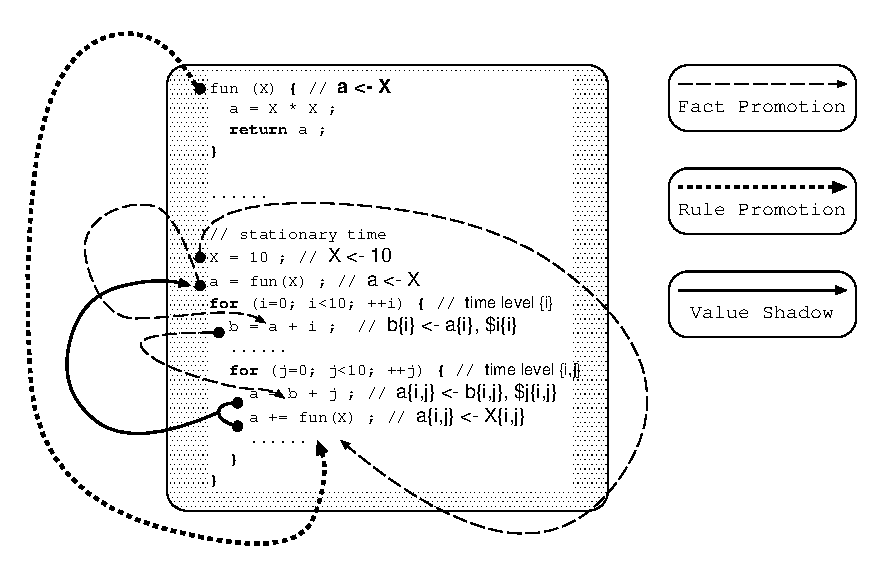
\includegraphics[width=5in]{promote}
%%  \centerline{ \epsfxsize=5in \epsfbox{promote}}
    \caption{Promotions in Loci}
    \label{promote}
  \end{center}
\end{figure}

There are two types of promotions in Loci: rule promotion and fact
promotion. Rule promotion handles computations that are independent of
the iteration level. Fact promotion handles the communications of
facts values across the iteration boundary. Figure~\ref{promote}
illustrates the promote concept in Loci. In Figure~\ref{promote}, Loci
specifications are compared to the conventional imperative programming
language. 

In Loci, stationary time rules are generic rules, they can
be used anywhere in the iteration hierarchy (i.e., computation
independent of time level). Rule promotion is to make
such rule usable in a given iteration. Basically, we will need to
match the facts name being produced in the iteration with the
rule. Since stationary time rules do not have time information
associated with them, we then append a time identity to every fact
involved in the rules (e.g., $A \gets B$ becomes
$A\{n\} \gets B\{n\}$). This is what rule promotion does. After rule
promotion, the promoted rule acts just as a time specific rule and can
be directly put in the iteration. Note, one rule promotion might
trigger more rule promotions once we look back in the searching.

Fact promotion is analogous to the variable scoping rule in most
programming languages. A variable defined in an outer block is
directly accessible to an inner block if it is not redefined in the
inner block. As in Figure~\ref{promote}, the value of $X$ and $b$ are
passed down to their child loops. Hence the $X$ in the $j$
loop are the same as the $X$ just before the $i$ loop; The $b$ in the
$j$ loop is the same as the $b$ in the $i$ loop. From the low level
memory management point of view, they occupy the same memory location
and have the same contents. The fact promotion is therefore created to
make Loci aware of such equivalence relationship between facts. Fact
promotion is represented by the {\it promote} internal
rule.\footnote{Note, this has no relation with rule promotion. As we
  pointed out, once a rule is promoted, it becomes a time
  specific rule. Therefore no special notation is needed.} Hence,
``$promote: A\{n\} \gets A$'' means $A\{n\}$ is just the $A$ from the
stationary time. As a note, we should remember that fact promotion
only happens between two successive levels. Thus if we want to relate
$A\{n,it\}$ to $A$, we will need two fact promotions. Namely 
``$promote: A\{n,it\} \gets A\{n\}$'' and 
``$promote: A\{n\} \gets A$.''
But if a variable is redefined in an inner block,
then it will shadow the value of the corresponding variable in the
outer block. For example in Figure~\ref{promote}, the $a$ in the $j$
loop shadows the $a$ before the $i$ loop. In Loci, if no fact
promotion exists between two facts with the same name (of course, with
time identity removed), then they are irrelevant. For example, if
there is no promote rule between $A\{n\}$ and $A$, then they are
independent facts. Or we can say $A\{n\}$ shadows $A$ in iteration
$\{n\}$. 

A serious Loci specifications for a real world application can have
rather complex rule and fact databases. For most of the facts, rule
promotion and fact promotion may both be applied. Therefore the
important problem is for a given fact, what promotion should we do,
and when and how should they occur. First we noticed, fact promotion
essentially denotes an equivalence relation between facts in different
time levels while rule promotion on a fact means that fact is time
specific and therefore independent. Hence, rule promotion and fact
promotion are mutually
exclusive. For any fact, we cannot have both rule promotion and fact
promotion. We must decide one of them if needed. 

The algorithm for promotion is already presented in
section~\ref{sec:algorithm}. Recall in section~\ref{sec:algorithm}, we
introduced the iteration volatile and static facts concept. If a fact
in an iteration is volatile, then we collect all possible rule
promotions for it. Otherwise if a fact in an iteration is static, we
promote the fact from the parent iteration. Combined with the
backgrounds in this section, it should be clear why we made such
decision and how we compute iteration volatile facts. 

We see in Figure~\ref{promote}, the $a$ in the $j$ loop shadows the
$a$ before the $i$ loop because $a$ is redefined in the $j$ loop. This
is exactly to say that the $a$ in the $j$ loop is a volatile variable
(or fact). Because $a$ is redefined (computed) in the $j$ loop,
therefore its value will change during each iterating within $j$, and
thus $a$ is volatile in the $j$ loop. And since $a$ in the $j$ loop
shadows any $a$ in any parent loops, $a$ is independent of its own in
the $j$ loop. Then we know fact promotion does not apply to $a$ in
the $j$ 
loop because it will establish equivalence relation to $a$ in the $i$
loop and then the $a$ in the stationary time. This is not what the
program mean, hence fact promotion does not
apply to iteration volatile fact. Since fact promotion does not apply,
we then will have to look for rule promotion for volatile fact. The
reason that we must consider rule promotion is because Loci is
declarative. We must look back to know how do we get a fact. We
will have to get {\it all} possible computations or the fact being
computed may miss some contents. Stationary time rules are independent
of time levels and can be used anywhere. We therefore need to consider
them too. And for this reason, rule promotions are necessary for any
volatile fact. It is also possible that a promoted rule coincides an
existing time specific rule. For example in the rule database there
are rules: ``$A \gets B$'', ``$A\{n\} \gets B\{n\}$.'' When we are on
$A\{n\}$, we will actually find two rules that computes it. One is
from the rule database directly and the other is from rule
promotion. But they really are the same. Hence in this case, we just
disregard the promoted rule. For any static fact like $b$ in the
$j$ loop, we do not know how to compute it in the $j$ loop. Thus
it must come from the parent loop. We then know fact promotion must be
added to any iteration static fact. 

As we described in \proc{Compute-Volatile-Facts} in
section~\ref{sec:algorithm}, a forward searching is used to compute
the iteration volatile facts. We have to use forward searching because
only volatile facts generate volatile facts and we know for an
iteration, some facts are guaranteed to be volatile. For example, in
Figure~\ref{promote}, for the $i$ and $j$ loops, we know for sure that
the iterators $i$ and $j$ are changing their value in each
iteration. Then we look forward and know $b$ in the $i$ loop is
volatile; $a$ in the $j$ loop is also volatile. This is a symmetric
process to the backward graph building phase. For the same reason as
rule promotion on volatile facts, we will need to gather {\it all}
possible computations. Stationary time rules might also involved. But
this time, we need to ``down promote'' the rule to stationary time to
collect possible reachable facts and promote the facts back to the
iteration as volatile facts. Therefore, we can understand the key
steps in~\proc{Compute-Volatile-Facts}. 

\begin{figure}[htbp]
  \begin{center}
    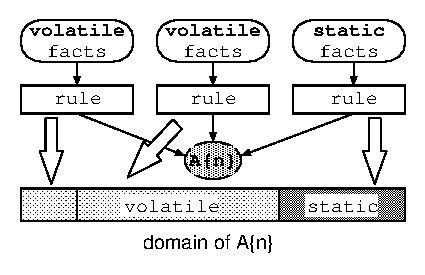
\includegraphics[width=2.75in]{volatility}
    %%  \centerline{ \epsfxsize=2.75in \epsfbox{volatility}}
    \caption{Partially Volatile Fact}
    \label{pvolatile}
  \end{center}
\end{figure}

As a final note for the promotion, we would like to distinguish
partially volatile facts and totally volatile facts. In
Figure~\ref{promote}, $b$ in the $i$ loop is a totally volatile fact,
while the $a$ in the $j$ loop is a partially volatile fact. In the $i$
loop, we can see that the contents of $b$ is updated entirely each
time in the iteration. Because $b=a+i$, and $i$ is changing each time,
hence $b$ must be changing completely. There are nothing else that
compute $b$, therefore we refer $b$ as totally volatile fact. In the
$j$ loop, $a$ is computed in two places. Notice in Loci, the
``+='' should be read as union instead of arithmetic addition. We see in
$a+=fun(X)$, the source $X$ is static. Therefore the part of $a$
computed from $fun(X)$ is always static. For this case, $a$ is
referred to as partially volatile fact. The concept can be visualized
as in Figure~\ref{pvolatile}. 

Note, a partially volatile fact is still a volatile fact because there
are still changing in its content. The difference is that we could
have two strategies and tradeoffs exist. From the time complexity
point of view, the computation of the static part is redundant and
could be singled out. Thus for example in Figure~\ref{promote}, the
computation of $a=fun(X)$ in $a+=fun(X)$ in the $j$ loop can be moved
to the initialization phase (along with $j=0$ in the code). Hence, we
can have less computations and the performance of the program will
improve. But from the space complexity point of view, the lifetime of
$a$ now extends to be the same as the $j$ loop. Therefore, we can
only safely release $a$ until we exit the $j$ loop. But if we instead
always recompute the static part of $a$ as the code in
Figure~\ref{promote}, then we may be able to release $a$ in each
iteration of $j$. Therefore we could save more space. However, this
choice is not decided in the dependency graph generation. It is
processed in the decomposition phase. The current Loci decomposer
chooses the time efficient strategy. 

\subsection{OUTPUT}
OUTPUT is a special fact in Loci. It is designed to facilitate file or
screen writing operations in iterations in Loci. Outputting is a side
effect and therefore we must handle it specially. Recall in
section~\ref{sec:algorithm}, in procedure~\proc{Init-Iter}, at
line~\ref{li:irule} we created a special internal looping rule whose
functionality is to hook the iteration rule set together. When we
creating the internal looping rule, we create an OUTPUT fact for that
iteration. For example, for iteration $\{n\}$, we create
OUTPUT$\{n\}$. This OUTPUT fact is attached to the internal looping
rule so that later in the decomposition, it will stay in the iteration
subgraph. If users want screen or file dump, they can create a rule
whose target is the OUTPUT fact. In the rule, users can do the desired
outputting actions. When such rules exist, the OUTPUT fact is said to
be activated. This is how Loci is informed of any outputting actions.
Currently, the OUTPUT stays in the advance part of an
iteration. Therefore, if it is activated, it gets executed every
time we in the advance part. Users can also control the frequency of
output. They can simply create a condition for the outputting
rule. For example, say outputting at every $50$th iteration. Thereby
reduce the outputting frequency. 

We can observe some properties of the OUTPUT fact. First, aside from
the internal looping rule, OUTPUT is always a target fact and never be
a source fact for a rule. Second, when activated, OUTPUT is always an
iteration volatile fact. This is because the contents of OUTPUT has to
change in the iteration, otherwise it is meaningless. It is just this
changes that we want to know and activated the OUTPUT in the
iteration. Since OUTPUT is a volatile fact, the same algorithms will
apply in building the dependency graph. Since OUTPUT is a volatile
fact, it is possible that we have a totally volatile OUTPUT or a
partially volatile OUTPUT. In the case of a partially volatile OUTPUT,
we will have some parts of the outputting that stay the same in the
iteration. Finally, we know that fact promotion never occur on any
OUTPUT facts since OUTPUT is volatile if activated. 

We now discuss how OUTPUT is handled in the dependency graph
generation. From the above discussion, we know when OUTPUT is
activated, it acts just as other volatile facts. Therefore the problem
is to determine whether it is activated or not for a given
iteration. Recall in the dependency graph generation, for each
iteration, we call~\proc{Compute-Volatile-Facts} to compute a set of
iteration volatile facts. Thus to know whether OUTPUT is activated is
just to check whether it is in the iteration volatile facts set. If it
is inside, then it is activated, otherwise it is deactivated. As we
discussed, for OUTPUT to be meaningful, it has to be volatile. Then if
it is volatile, it must be activated in the iteration. Also as we
discussed, OUTPUT is always a rule's target. Thus in the backward
searching, we have no way to reach it. Therefore, if it is activated,
we will have to add it into the initial searching requests of an
iteration. This is what line~\ref{li:output1} and~\ref{li:output2}
mean in the~\proc{Init-Iter} procedure. 


\section{The Analysis of Algorithm}
Time complexity analysis.\\
To be written\dots

\end{document}
